 \documentclass{article}

% if you need to pass options to natbib, use, e.g.:
% \PassOptionsToPackage{numbers, compress}{natbib}
% before loading nips_2016
%
% to avoid loading the natbib package, add option nonatbib:
% \usepackage[nonatbib]{nips_2016}

\usepackage[final,nonatbib]{../LaTeXStyleFiles/nips_2016}

% to compile a camera-ready version, add the [final] option, e.g.:
% \usepackage[final]{nips_2016}

\usepackage[utf8]{inputenc} % allow utf-8 input
\usepackage[T1]{fontenc}    % use 8-bit T1 fonts
\usepackage[colorlinks]{hyperref}       % hyperlinks
\usepackage{url}            % simple URL typesetting
\usepackage{booktabs}       % professional-quality tables
\usepackage{amsfonts}       % blackboard math symbols
\usepackage{nicefrac}       % compact symbols for 1/2, etc.
\usepackage{microtype}      % microtypography
\usepackage{amsmath}
\usepackage{tikz}
\usetikzlibrary{positioning}
\usetikzlibrary{shapes.geometric}
\usetikzlibrary{calc}
\usetikzlibrary{circuits.logic.US}

\tikzset{
  multiplexer/.style={
    draw,
    trapezium,
    shape border uses incircle, 
    shape border rotate=270,
    minimum size=18pt
  }
}

\bibliographystyle{ieeetr}

\title{Project Proposal}

% The \author macro works with any number of authors. There are two
% commands used to separate the names and addresses of multiple
% authors: \And and \AND.
%
% Using \And between authors leaves it to LaTeX to determine where to
% break the lines. Using \AND forces a line break at that point. So,
% if LaTeX puts 3 of 4 authors names on the first line, and the last
% on the second line, try using \AND instead of \And before the third
% author name.

\author{
    Kyle~Daruwalla \\
    Department of Electrical and Computer Engineering \\
    University of Wisconsin -- Madison \\
    \texttt{daruwalla@wisc.edu} \\
    \And
    Akhil~Sundararajun \\
    Department of Electrical and Computer Engineering \\
    University of Wisconsin -- Madison \\
    \texttt{asundararaja@wisc.edu} \\
}

\begin{document}

\maketitle

% Each section (including abstract) has its own .tex file
% The name of the .tex file corresponds to the section title
% e.x. The subsection in the Introduction on FPGAs is called
%      intro-fpga.tex
% \input{filename} is equivalent to pasting in the raw text
% from filename.tex.
% Try to edit the filename.tex files and not proposal.tex.
% This avoids conflicts most of the time.

\section{Introduction}
Machine learning systems tackle problems ranging from content filtering and recommender systems to object recognition and text classification.  In recent years, advances in deep learning have led to finding better classifiers for these problems.  In deep learning, feature extraction is performed automatically by using many layers of neural networks; each layer involves passing inputs of the previous layer through a nonlinear activation function.  Compositions of successive layers can thus correspond to learning nonlinear decision boundaries, which has contributed to successes in image classification  and speech recognition.  Training of deep neural networks is performed using the stochastic gradient descent (SGD) algorithm, but the inherently serial nature of SGD has led to exploration of potential speedups through parallelized hardware.  In this project, we seek to investigate how the computational cost per iteration of training a deep neural network depends on the hardware architecture being used. 

\subsection{Field-Programmable Gate Arrays}
Even though learning algorithms are inherently serial, speedup might be possible by using specialized hardware to reduce the cost per iteration.

Field-programmable gate arrays (FPGAs) are reconfigurable hardware chips. An FPGA is comprised of \textit{slices}, which are the fundamental hardware unit from which any designed hardware is constructed. Each slice is comprised of \textit{look-up tables} (LUTs) and \textit{flip-flops} (FFs). When reporting the resource consumption of a particular design, it is common to report the metric in terms of slices or LUTs+FFs.

Hardware on an FPGA is designed using a \textit{hardware description language} (HDL). The most common HDL is Verilog. While Verilog shares some syntax with C, it should not be confused for a sequential programming language. HDLs allow a designer to spatially describe the hardware.

FPGAs are commonly used for real-time control, because the design freedom they offer allows for lean, efficient controller design. Furthermore, designs are not hampered by hardware limitations, because the designer can create any hardware he desires. As the boundary between control theory and optimization has blurred, FPGAs have become suitable hardware platforms for machine learning algorithms such as neural networks \cite{wang2008} \cite{skodzik2013}. Similarly, FPGAs are an attractive option to make object-recognition algorithms real-time \cite{ahn2015}.

While previous work has largely focused on deployment of neural networks on FPGAs, this project will focus on the training phase. Specifically, can FPGAs be utilized to build efficient parallel hardware to speedup the lengthy training process for convolutional neural networks?

\section{Design Methodology}
In order to perform an effective comparison between software implementations of CNNs and hardware implementations, we use TensorFlow, MATLAB, and Xilinx FPGAs. TensorFlow is used to train software implementations of a given CNN structure for CIFAR-10. These CNN implementations were trained and tested on a traditional CPU. A hardware implementation of the CNN has been created for Xilinx FPGAs in Vivado. Simulations have been performed to verify its functionality and collect timing characteristics, while an equivalent MATLAB model verifies its convergence.
\subsection{TensorFlow Baseline}
\textit{Information on TensorFlow implementation on EC2. Talk about CPU baseline. Talk about speed up using GPU and Hogwild!}
\subsection{Convolutional Neural Networks on FPGAs}
\textit{Information on implementing a neural network on FPGA}
\subsection{MATLAB Verification}
While our hardware implementation is serially equivalent to a traditional software implementation for a CNN, it does use limited precision. We implemented a limited precision CNN model of the hardware in MATLAB to verify its convergence.

This was achieved by using a custom quantization function to limit the precision of the numbers used by MATLAB. Using a custom function allowed us to have tight control of the rounding scheme, and it is faster than using the object-oriented fixed-point model in MATLAB.

Similar to the TensorFlow and hardware, the MATLAB simulation is also trained using mini-batch stochastic gradient descent with a batch size of 128 (same as TensorFlow). The purpose of this simulation was to emulate training the hardware on the same dataset as TensorFlow verify the hardware's convergence. It was not intended to be used for a timing comparison.

\section{Results}
We perform a total training time comparison between TensorFlow implementations and the FPGA hardware. Additionally, we perform a loss convergence comparison between the simulated hardware in MATLAB and the TensorFlow implementation.

\subsection{Total Runtime Results}
After designing the hardware, we simulated the Verilog in Vivado to find the total number of clock cycles to train one batch of mini-batch SGD. We the multiply this value by the operating clock period of the FPGA to determine to absolute time measurement to train a single batch for various clock frequencies. Lastly, we multiply that value by the total number of batches to find the total training time for the given FPGA implementation.

Fig. \ref{fig:total-runtime-plot} displays a comparison of the total training time in minutes between the TensorFlow implementations and the FPGA implementation at varying clock frequencies. As can be seen in the plot, the FPGA needs to be run at 50 MHz minimum to notice any speed up.
\begin{figure}[ht]
	\centering
	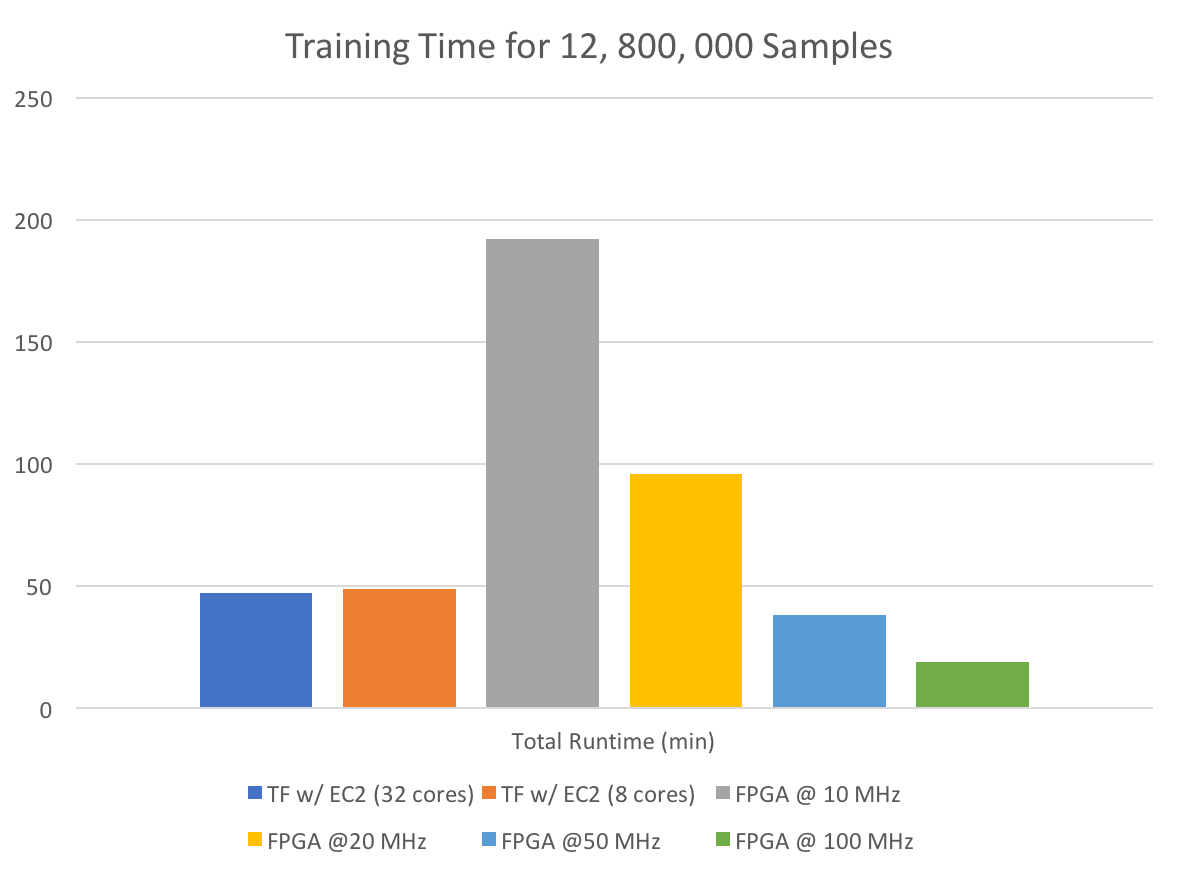
\includegraphics[scale=0.6]{total_runtime_plot.png}
	\caption{A comparison of training time for 12,800,000 samples}
	\label{fig:total-runtime-plot}
\end{figure}

Notice that the TensorFlow implementation notices little to no speed-up going from 8 to 32 cores. This illustrates the lack of potential in current traditional strategies for achieving speed-up by increasing the number of cores or machines. The FPGA implementation, however, scales linearly with frequency. The largest deterrent of running the FPGAs at 100 MHz or higher, is the lack of on-chip resources. Specifically, attempting to fit an entire CNN on a single FPGA introduces too much global routing overhead, which leads to a lower maximum clock frequency. We suspect that by partitioning the neural network by layers onto multiple FPGAs, the hardware will be able to run at the higher frequencies required to achieve speed-up.

\subsection{Loss Convergence Results}
We trained the MATLAB simulation of the hardware using the same dataset as the TensorFlow implementation to verify its convergence. Fig. \ref{fig:loss-plot} illustrates the convergence of the loss versus number of samples processed. Clearly, the loss converges, but it coverges to a worse loss than the full precision TensorFlow implementation.
\begin{figure}[ht]
	\centering
	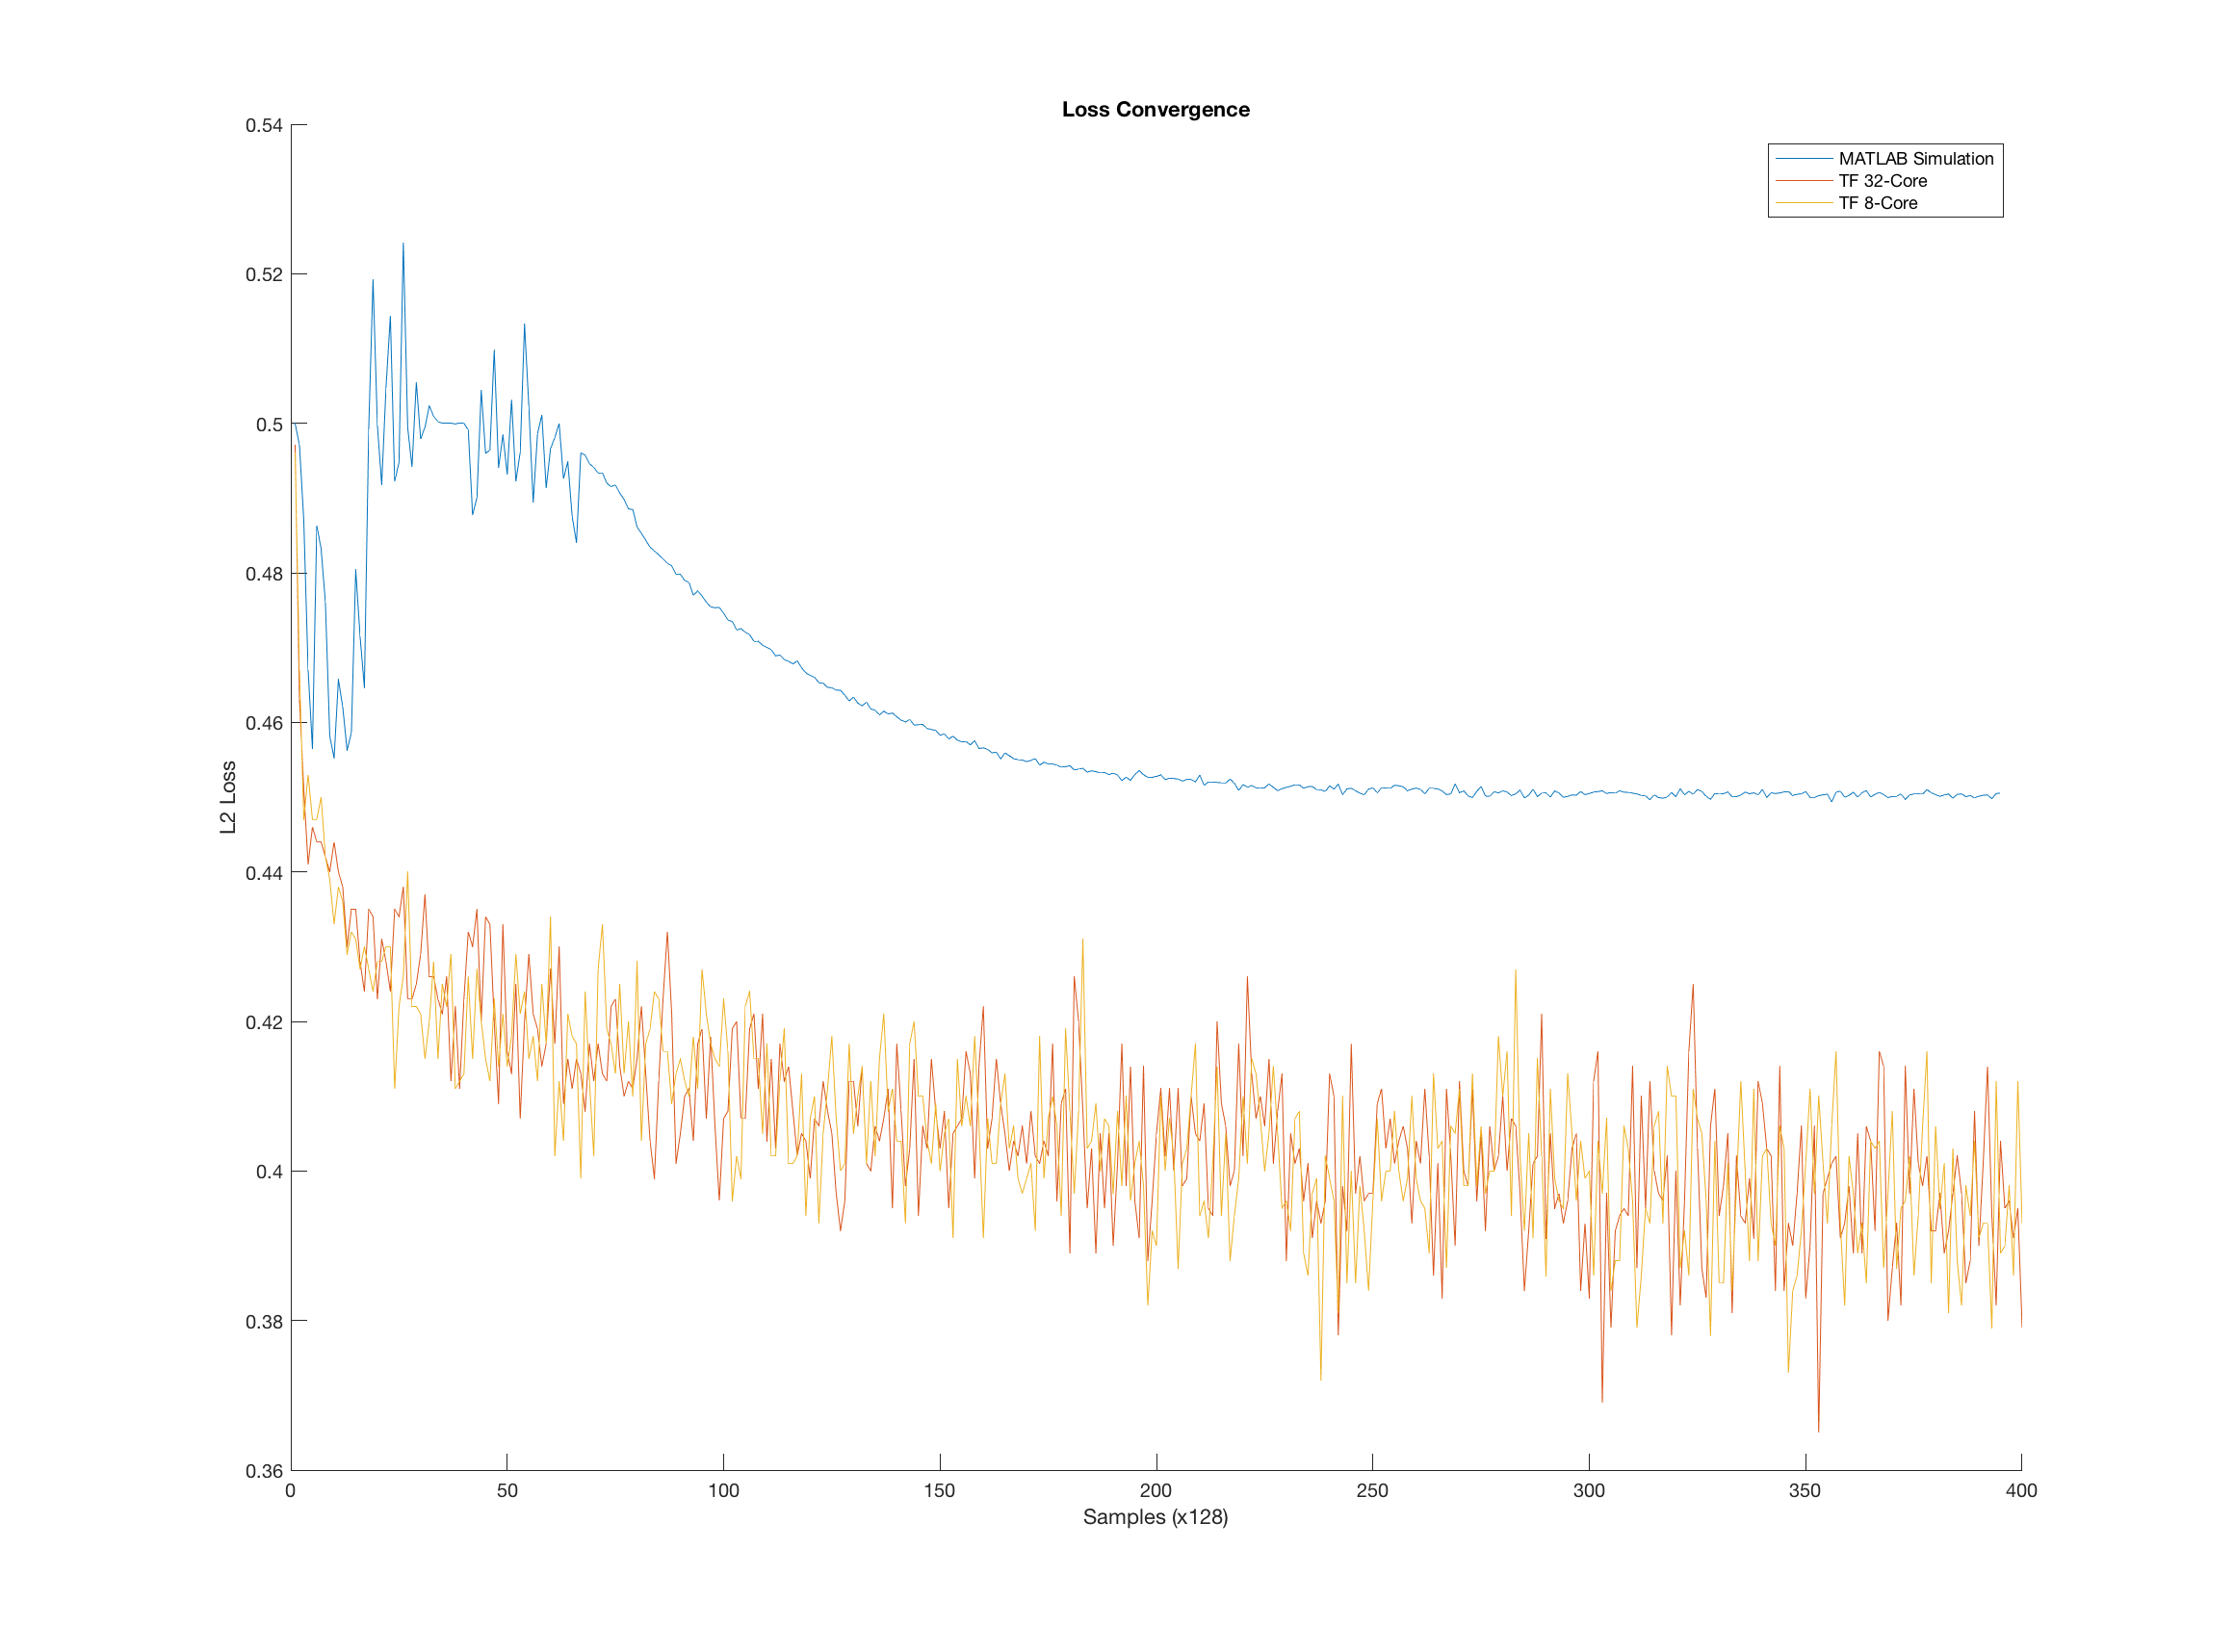
\includegraphics[scale=0.17]{../all_loss_plot.png}
	\caption{The loss versus number of samples processed for the MATLAB and TensorFlow implementations}
	\label{fig:loss-plot}
\end{figure}
The purpose of this analysis was primarily to verify that the hardware is capable of producing a trained CNN. Initially, we expected our loss convergence plots to look similar to Gupta et al. \cite{limited-precision}. However, our plot shows a noticeable difference in the loss value that each implementation converges to. We expect that this is due to the difference in size between our network and the networks implemented by Gupta et al. Since our CNN contains siginificantly less layers and learned parameters, the effect of losing a bit of precision is amplified. In a larger network, the layers can work together to mitigate the effects of losing precision. We believe this discrepancy in the loss convergence plots lends creedence to the need to explore the effects of limited precision training more in depth.

\section{Conclusion}
Our results show that FPGAs are a viable option for speeding up the training phase for CNNs. However, we also note that these implementations are constrained by the resources available, and thus, FPGA implementations are only useful if the network can be partitioned. In particular, training a small to medium sized networks on a single CPU or GPU is likely a better option than an FPGA implementation. However, as the input data and the network depth scales up, the benefits of CPU implementations fail to deliver speed-up. Particularly, at the scale of data centers like Microsoft \cite{project-catapult}, an FPGA implementation offers the necessary speed-up while still being more power efficient than an equivalent GPU offering.

Furthermore, our loss convergence results illustrate the need to explore limited precision training more deeply. Currently, neural network designers add controlled noise to the data or model (via dropout) in order to increase the model robustness. We would like to explore using quantization error to introduce this noise. The properties of quantization error can be controlled and bounded via varying rounding schemes. Moreover, the benefits of quantization and limited precision are two-fold -- first, controlled noise can make the model more robust if inserted intelligently; second, the reduced bit length leads to faster hardware and more resources on-chip to create parallel execution units.

In summary, this project illustrates a promising direction for further exploration. In the future, we would like to implement partitioning networks across several FPGAs to increase the clock frequency and number of parallel execution units, as well as understand the effects of quantization and limited precision on the robustness of CNNs. We conclude that FPGAs are a suitable candidate for speed-up when the networks and datasets are sufficiently large, and when aggregate power consumption is costly.

\newpage
\nocite{*}
\bibliography{references}

\end{document}
